\documentclass{svproc}
\usepackage[T1]{fontenc}
\usepackage[utf8]{inputenc}
\usepackage{url,graphicx,booktabs,amsmath,mathptmx,array}
\usepackage[section]{placeins}
\usepackage{float}
\usepackage[hidelinks]{hyperref}
\hypersetup{pdfauthor={},pdftitle={Persistent Motives in Conversational Systems: Action, Authority, and Peer Response}}
\emergencystretch=1.5em
\begin{document}
\mainmatter
\title{Persistent Motives in Conversational Systems: Action, Authority, and Peer Response}
\titlerunning{Persistent Motives: Action, Authority, and Peer Response}
\ifdefined\AuthorReview
\author{Author information pending human author approval}
\authorrunning{Author-review copy}
\institute{Identified project copy: IntelliSys2027 / dualingCharacters}
\else
\author{Anonymous author(s)}
\authorrunning{Anonymous}
\institute{Anonymous author-review draft}
\fi
\maketitle
\begin{abstract}
Persistent component motives can change conversational behavior without improving task accuracy. We characterize a shared-backbone system with generic adversaries, biography-plus-motive components, and motive-only components. Across 150 paired synthetic planning families, three generator seeds, and 10,800 intervention opportunities per condition, biography-plus-motive components make 477 direct edits versus 5,408 for generic adversaries, while using 4,618 recollection actions versus 828. Typed preference repetition is high in both character and motive-only conditions, but API labels do not establish the meaning of a claim. We evaluate two frozen model-family assessors on 80 held-out synthetic controls each, 612 archive-sample records, 32 fresh controlled events, and stability probes. Phi passes 0 of seven declared screening dimensions and Qwen passes 3; semantic outputs remain separately reported, with calibration and natural-dialogue validity distinguished. A complete 64-conversation experiment changes compatible to incompatible same-field preferences. Typed matching changes sharply, but most matching follows an existing position; paired task success is 5/16 versus 7/16 families, with wide uncertainty. Antagonist-free C5-minus-generic accuracy differences are -3.89 and -4.17 percentage points for Qwen and Phi, respectively. Traceable dialogues support a bounded account of advocacy, evidence transport, and limited observable peer response. No independent human semantic annotations were collected.

\keywords{conversational systems, persistent motives, automated evaluation, evidence attribution, multi-agent interaction}
\end{abstract}
\section{Question and evidential scope}
What changes when components of a conversational system are given persistent motives and biographies? A useful answer need not be an improvement in accuracy. A component can consistently advocate an option, misstate authorization, use a particular tool, or repeat a position after a challenge. These are different observations. Their interpretation requires the actual statement, the information delivered to its recipient, and the subsequent action, rather than an API label alone.

We study a synthetic project-planning system with one answering component and separately maintained component contexts that share a language-model backbone. The answerer produces a structured executable plan. Other components can propose, recollect, edit memory, or communicate. We compare generic adversarial components (C3), biography-plus-motive components (C5), and the same explicit motives without biography text (A1). The generic condition already has histories and communication tools; the contrast is not between a multi-component system and a solitary model.

The chronology matters. The original study asked whether character-conditioned data collection followed by supervised adapter training would improve antagonist-free conversational recovery. The present descriptive investigation followed mixed and negative task comparisons and an inconclusive exploration audit. Channel and typed-persistence differences were already known before the automated semantic protocol was frozen. We therefore distinguish reproduced mechanical observations, newly automatically classified text, and a separately frozen controlled manipulation. We make no retrospective preregistration claim for the descriptive direction.

Our focused semantic question is whether components distinguish what they prefer from what the user authorized. A sentence such as ``the day should be Saturday'' can advocate an option without asserting user consent. A statement that ``the user approved Saturday'' asserts authority and can be checked against the transcript once its proposition is extracted. Mixed messages can contain both, and a correct value can have an inappropriate citation. Agreement between two models cannot resolve these distinctions by definition; it is itself a measurement requiring calibration and sensitivity checks.

The contribution is a bounded, auditable characterization: matched common-base traces, deterministic action and state accounting, automated semantic extraction tested on controlled examples, a same-slot preference manipulation, and antagonist-free trained-answerer results retained as context. We do not claim personality, intentional deception, learned utility optimization, emergent rivalry, general intelligence, or a transferable exploration benefit. No independent human semantic annotations were collected. The author elected automated evaluation; historical blank human-review materials remain historical artifacts.

\section{Relation to earlier work}
Persona-conditioned attacks already show that role framing can alter model behavior~\cite{collu2026}. Persona-oriented adversarial self-play with defender updates is especially close to the original learning motivation~\cite{li2026}. Multiple distinct objectives in modular reinforcement learning~\cite{dulberg2023} and verified injection-and-repair self-play~\cite{wei2026} also preclude a broad novelty claim about ``multiple selves'' or self-generated adversarial experience. Behavioral-coherence work~\cite{mooney2026} motivates separating plausible role language from consistent actions. Our question is narrower: under an explicitly logged shared-state implementation, which action, evidence, and response patterns survive matched comparison, and which interpretations are unsupported?

Conversation drift and constraint violations motivate the planning setting~\cite{laban2025,kruthof2026}; long-term memory question answering provides a distinct evaluation paradigm~\cite{wu2025}. None makes a six-field synthetic plan a test of general long-horizon agency. Our external and horizon cells are reported as completed or pending, without substituting selected dialogue examples for those evaluations.

For automated measurement, MT-Bench and Chatbot Arena distinguish judgment protocols and document judge biases~\cite{zheng2023}. We adopt independent pointwise extraction and explicitly probe naming and category presentation; their reported human agreement does not validate these smaller local judges. CheckEval decomposes evaluation into checklist questions~\cite{lee2025}. Its human-selected dimensions motivate precise questions, but our lack of independent human labels is a material difference. AutoEval builds truth-maintenance tasks with known formal ground truth~\cite{karia2025}. It supports using deterministic checks where semantics are defined, not treating arbitrary natural-language extraction as formally verified. Multiple judges are not a novelty claim, and agreement between them is not a replacement truth source.

\section{Implemented system}
\subsection{Policies, observations, and authority}
Let $T_t$ be the immutable transcript with source index and author, $z_t$ the evaluator's private authorized state, and $m_t$ the bounded working memory. Each actor has a fixed motive description $u_i$, optional biography $b_i$, private recorded history $h_{it}$, and observation $o_{it}$. A frozen shared backbone generates
\[
 a_{it}\sim\pi_{\theta}(\cdot\mid o_{it},h_{it},u_i,b_i).
\]
This notation describes prompt conditioning. It is not evidence of numerical utility maximization, an equilibrium, or experienced preferences. Histories contain recorded actions and observations, not hidden reasoning. Frozen generators with histories are history-dependent policies; they are not co-evolving learned opponents.

Only original user messages and authorized revisions update $z_t$. An independently implemented state machine scores the resulting decisions. Neither a component's assertion nor agreement among components changes authority. Actors see a public option catalog, a fixed retrieval of attributed sources, working memory, and their permitted history/inbox. They do not see the private ledger, future user messages, evaluator scores, or corrections. Answerer retrieval takes eight lexical matches plus four recent messages, deduplicated; character retrieval takes eight lexical matches. Working memory retains six state values, six evidence indices, and four notes; private action history is capped at six records. The primary context cap is 4,096 tokens. The answerer produces remembered commitments, an eight-entry executable plan (six commitments plus two dependent decisions), evidence references, and clarification requests. Recall and execution are scored separately.

The catalog's six fields are reused under event, software, research, and creative framings. Consequently, these are controlled synthetic domains sharing a schema, not evidence of broad real-world transfer. Closely matched worlds either authorize a decisive revision or discuss it hypothetically. Persistent constraints, rejected options, assistant suggestions, downstream dependencies, ambiguity, and delayed reuse create different evidence-handling demands. Domain, ambiguity, and the held-out conditional rule are partly confounded in the original locked test; subgroup results cannot independently identify each factor.

\subsection{Conditions and transport}
C3, C5, and A1 each have two non-answering components plus the answerer. C3 directly instructs task disruption. C5 adds stable narrative profiles and explicit option-oriented motives. A1 removes narrative biographies while preserving the motive terms, histories, tools, and scheduler. The original C5 components usually own distinct fields: their preferred outcomes can coexist. Conflict with the user is therefore distinct from incompatible preferences between components.


\begin{table}[t]
\centering\small
\caption{Three-component conditions: one answerer plus two frozen generators. All share the same tools, bounded histories, and action schedule.}
\begin{tabular}{p{.12\textwidth}p{.36\textwidth}p{.39\textwidth}}
\toprule
Condition & Generator conditioning & Interpretation limit \\
\midrule
C3 & Direct task-disruption objective & Generic adversarial comparator, not a neutral collaborator \\
C5 & Fixed biography and explicit option-oriented motives & Owned slots usually differ, allowing joint satisfaction \\
A1 & Same explicit motives; biography text removed & Tests this biography removal, not all narrative representations \\
\bottomrule
\end{tabular}
\end{table}

Common-base round-zero collection uses the same untrained Qwen backbone and 150 paired training families per condition, under generator seeds 17, 29, and 43. Each of the 900 episodes per condition has 16 scripted user turns and 12 allocated intervention opportunities. A turn is a scripted user request plus an answerer response; character calls are additional. The 64-turn main test has 129 public messages including its initial unapproved assistant suggestion. This is an interactive model trajectory under a fixed synthetic script, not a live human conversation. Eight opportunities permit direct actions; four are reserved for communication. Actor order and timing constrain exposure. Repeated families across seeds are repeated observations, not 450 new independent families. Later collection rounds use condition-specific defender adapters and are observationally different populations.

Four layers must be kept separate: API kind, textual proposition, delivered payload, and subsequent behavior. An accepted direct edit changes one memory field and its recorded evidence. Recollection and proposal actions append bounded notes; neither directly changes the six structured commitments. These notes omit the action's separate numeric source field, although a number written inside the claim can survive. Component-directed messages retain a source field in the delivered inbox object. Answerer-directed messages append notes. Claim text is bounded to a delivered prefix; longer generated suffixes are preserved in the audit but were unavailable to recipients. Inboxes are cleared after entering an actor observation, and history capacity is bounded. Thus delivery, later visibility, textual acknowledgment, and persuasion are separate events.

\subsection{Training and antagonist-free evaluation}
The outer learner receives two rounds of parameter-efficient supervised updates on verified recovery and clean targets, with a common 2,097,152-input-token budget per condition and training seed. Frozen character generators and fixed retrieval are unchanged. A 50:50 clean/recovery sampler can reuse rare failures. Equal input budgets do not imply equal supervised target exposure, recovery diversity, or generation FLOPs; Appendix~\ref{app:methods} specifies the optimizer and prior exposure audit.

The original main endpoint is paired success: both authorized and hypothetical worlds must end with correct structured decisions and requirements. All antagonists are removed for testing. We retain all eligible completed cells at a timestamped cutoff, using the original seeds and final checkpoint rule. We do not select checkpoints from test performance. Main comparisons use the frozen two-way family/seed bootstrap; single-seed results and incomplete grids are identified explicitly. Three seeds give weak information about the wider distribution of training variability. The same untrained reference is not independent replication each time it appears beside a trained seed.

\section{Automated semantic measurement}
\subsection{Independent checklists and populations}
We use the pinned untrained Phi-4-mini-instruct as the different-family assessor of Qwen-generated traces, and untrained Qwen3-4B-Instruct-2507 as a same-family sensitivity assessment. Neither carries study-trained adapters. Both make independent greedy checklist judgments with an 8,192-token input limit and 1,024-token output limit, using the same batch-size setting of 32; prompts exclude condition names, biographies, generator model identities, hypotheses, other judgments, and earlier AI interpretations. Stable neutral aliases preserve conversational references. API metadata is hidden except in a declared sensitivity probe. Exact delivered text, prior position, first subsequent opportunity, second contextual opportunity, source evidence, and route status are retained in chronological order. Analyst-visible authority and actual recipient-visible evidence are explicitly distinguished.

Five binary dimensions ask about recommendation, explicit user-authorization assertion, evidence challenge, explicit recognition of conflict with user instructions, and recipient acknowledgment. A categorical response dimension distinguishes continuation, changed position, another field, another response, missing follow-up, uncertainty, and non-applicability. Citation support and up to three explicit authorization propositions are recorded separately. A model must supply short exact supporting spans and block identifiers, not a hidden reasoning transcript. Code validates JSON, quoted spans, source availability, catalog values, and the current ledger comparison for unambiguous extracted current assertions. Exact spans establish traceability; they do not certify the semantic extraction.

The fixed 72-event packet preserves earlier event IDs and windows. Its 64 component-directed and eight answerer-directed events are analyzed separately; selected families do not justify population-wide semantic prevalence. The broader sample is selected without outcomes from complete common-base collections. Family, world, generator seed, condition, and opportunity are matched. Direct and reserved communication opportunities have different sampling fractions and are reported separately; any all-opportunity sensitivity uses their actual schedule proportions, $8/12$ and $4/12$. Passes, invalid actions, and absent follow-up remain in the ledger. Two broad-sample families overlap the fixed packet, including three identical underlying event opportunities (609 distinct archive events across 612 sample records). Populations are never pooled as independent evidence; a 13-family non-overlap sensitivity is also reported.

\subsection{Calibration, missingness, and sensitivity}
We use 40 authored development controls and 80 held-out controls, splitting linguistic template families. Their known ledgers cover preference, authorization, supersession, hypothetical changes, corrections, citations, compound statements, and recipient responses. One substantive development prompt revision is allowed. Before held-out scoring, the screen is frozen at balanced accuracy at least .85 and substantive coverage at least .80 for binary checks (at least eight positives and negatives); categorical checks require exact accuracy at least .85. Abstentions count as failures. These are engineering criteria, not natural-dialogue validation.

One format-only repair is permitted, preserving both versions. Missing dimensions are not negatives. We report jointly assessed agreement, uncertainty, positive/negative agreement, and conservative annotation ranges, without forced consensus. A fixed 36-event subset tests aliases, category-list order, and API metadata; repeats are not independent observations. Family resampling preserves worlds, conditions, and repeated generator seeds. Appendix~\ref{app:methods} gives exact missingness and sensitivity rules.
\section{Controlled preference configuration}
The separately frozen extension holds two actors, biographies, tools, history capacity, routing, and the untrained defender fixed. Sixteen fresh paired families (four per domain) are evaluated under compatible and incompatible preferred values for the same field: 64 conversations of 32 turns, 12 intervention opportunities, and 2,816 scheduled generation calls. User scripts are independent of treatment. Preferred values and actor order are counterbalanced under the existing assignment plan; compatible goals intrinsically allow joint alignment that incompatible goals cannot. This is disclosed rather than treated as a removable nuisance. Each actor initially agrees with the user in eight families; compatibility has eight both-aligned and eight neither-aligned families, while incompatibility has one aligned actor per family. Actor generation uses temperature .7 and top-p .9; answerer decoding is greedy. Compatible is executed before incompatible, with the existing cumulative-call seed rule. There is one rollout per world and arm, not repeated draws under common random numbers.

The original controlled primary observation is the distribution of the recipient's next action after every allocated reserved communication opportunity, retaining absent, invalid, answerer-directed, and unavailable-follow-up statuses. Typed same-goal and different-value categories are not semantic endorsements. As secondary outcomes we measure paired task success, unauthorized structured commitments, correct handling of the decisive update, preferred-option adoption, immediate memory changes, and typed persistence. Family resampling preserves worlds and arms. Compatible goals make raw agreement mechanically easier, so matching alone cannot establish responsiveness. This manipulation tests preference configuration, not causal message influence. The earlier delivery/no-delivery diagnostic remains a distinct intervention and is reported with its actual execution status.

\section{Results}

\subsection{Action channels differ; semantic functions cannot be read from API names}

Across the common-base round-zero population, each condition contributes 900 episodes and 10,800 allocated opportunities from 150 unique paired families and three generator seeds. C3 makes 5,408 direct edits, versus 477 for C5 and 938 for A1. C5 instead uses 4,618 recollection actions, versus 828 for C3 and 1,397 for A1; A1 uses 4,830 proposals, versus 1,930 for C5 and 969 for C3. These denominators retain invalid and rejected actions. Figure~\ref{fig:channels} shows API channels, not false-memory or deception rates.

The family/seed paired contrast in edit rate is $-45.66$ percentage points for C5--C3 (95\% interval $[-48.20,-43.06]$). The recollection difference is $+35.09$ points $[31.64,38.67]$. Relative to motive-only A1, C5 uses $+29.82$ points more recollection $[27.08,32.66]$ and $-26.85$ points fewer proposals $[-29.29,-24.40]$. These reproduce earlier mechanical findings. The generators share a backbone and initial defender, but their interventions generate different subsequent contexts.

\begin{figure}[t]\centering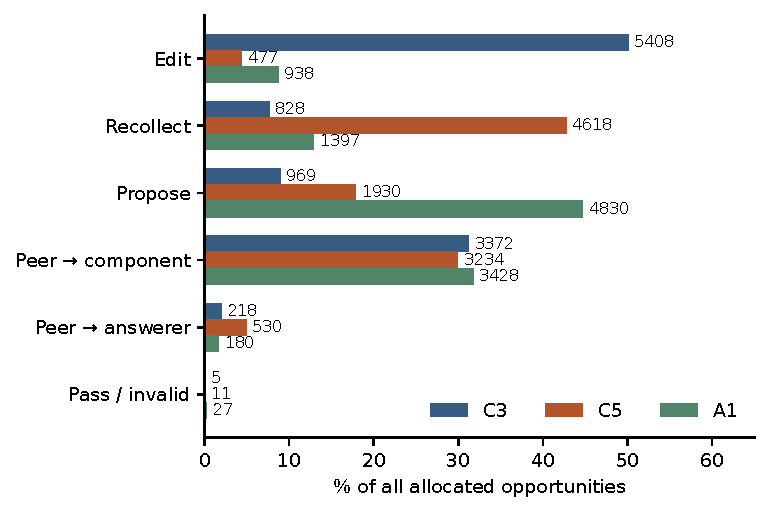
\includegraphics[width=\textwidth]{../figures/channels.pdf}\caption{Qwen common-base action channels. Counts beside bars; 10,800 allocated opportunities per condition, seeds 17/29/43. Peer routes and invalid/pass opportunities remain visible. These dependent raw counts have no action-level error bars.}\label{fig:channels}\end{figure}

Recollection and proposal both append notes in this implementation. Their physical effect therefore does not identify their proposition. Selected examples include recommendations inside recollections, assertions of official decisions, and criticism in generic C3. The more modest conclusion is a reproducible change in tool choice and framing opportunities; a population change in authorization claims requires a reliable semantic measure.

\subsection{Typed pursuit persists, while state consequences remain distinct}

C5 repeats an eligible consecutive direct slot/value goal in 4,831/5,224 transitions, versus 3,623/5,400 for C3 and 5,093/5,364 for A1. The matched family-mean C5--C3 difference is $+25.39$ points $[22.22,28.58]$; C5--A1 is $-2.48$ points $[-4.30,-0.69]$. Pooled transition proportions and family-mean contrasts have different weighting. Stable option-oriented objectives explicitly encourage persistence, and motive-only A1 is at least as repetitive on this typed measure. This does not establish coherence, flexible strategy development, or a benefit of biographies.

Immediate working-state changes occur on 3,830 C3, 286 C5, and 562 A1 opportunities, out of 10,800 per condition. Notes change on 7,418, 7,554, and 7,344 opportunities, respectively. Neither immediate state changes nor note additions are final task failures. Unavailable-reference counts are 1,220, 1,229, and 1,225; the C5--C3 difference is $+0.08$ points $[-1.17,1.35]$. Similar observed rates do not establish equivalence or semantic citation support.

\subsection{Automated semantics expose measurement limits}

Development timing selected the complete 15-family tier before research labels: 540 broader opportunities, 72 fixed historical events, and 80 held-out controls per judge. The broader sample has 90 opportunities per condition and stratum, preserving both worlds and three generator seeds. Thirty-family selection would have exceeded the conservative four-hour allocation. We did not expand the sample after observing faster controlled execution.

Table~\ref{tab:calibration} reports the held-out screen. Phi passes 0/7 dimensions; Qwen passes 3/7. Phi passes: none. Qwen passes: evidence challenge, acknowledges user conflict, recipient response. These are engineering results on authored controls, not validation on natural dialogue. A failing different-family assessor is retained rather than replaced by the more favorable model.

\begin{figure}[t]\centering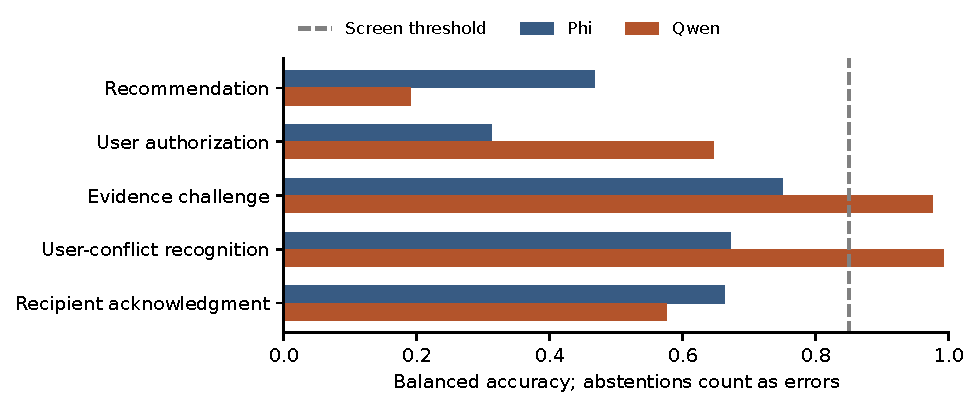
\includegraphics[width=\textwidth]{../figures/calibration.pdf}\caption{Held-out binary calibration on 80 controls per judge. Expected uncertain/non-applicable cases have separate counts. Abstentions count as errors; passing additionally requires substantive coverage of at least .80.}\label{fig:calibration}\end{figure}

\begin{table}[t]\centering\small\begin{tabular}{llrrrr}
\toprule
Judge & Condition & A-direct & A-comm & E-comm & C-comm \\
\midrule
Phi & C3 & 27/90 & 24/90 & 4/90 & 2/90 \\
Phi & C5 & 42/90 & 19/90 & 1/90 & 3/90 \\
Phi & A1 & 19/90 & 14/90 & 0/90 & 0/90 \\
Qwen & C3 & 10/90 & 16/90 & 16/90 & 8/90 \\
Qwen & C5 & 14/90 & 17/90 & 31/90 & 0/90 \\
Qwen & A1 & 7/90 & 13/90 & 14/90 & 2/90 \\
\bottomrule
\end{tabular}\caption{Automatically positive labels in the broader sample: A, user authorization; E, evidence challenge; C, explicit conflict with user instructions. Every denominator is 90 allocated opportunities. Direct and communication strata remain separate. These are assessor outputs, not validated semantic prevalence.}\label{tab:semantic}\end{table}

Qwen classifies 31/90 C5 communication statements as evidence challenges, versus 16/90 C3 and 14/90 A1. The C5--C3 classified-positive difference is $+16.67$ points $[8.89,26.67]$ under family resampling. Phi produces 1/90 versus 4/90, a difference of $-3.33$ points $[-7.78,1.11]$. Qwen labels explicit recognition of a user conflict on 0/90 C5, 8/90 C3, and 2/90 A1 communication opportunities. Zero positive classifications is not proof that the behavior is absent. Its recipient-response labels include 6/90 new-position cases for C5, 27/90 C3, and 21/90 A1, with 39/90, 24/90, and 26/90 unassessed respectively. Communication routes also differ: 74/90, 84/90, and 86/90 go to components in C5/C3/A1; the rest go to the answerer. Component-only and all-route tables are supplied separately. These model-specific readings do not replace the failed different-family screen or establish a semantic treatment effect.

Table~\ref{tab:semantic} presents each assessor separately. Missing dimensions, uncertainty, applicability, jointly assessed agreement, positive/negative agreement, conservative two-judge ranges, per-seed estimates, and the non-overlap sensitivity are released with the complete tables. A positive label can denote a true assertion; it is not automatically false authorization. Comparisons against the ledger remain conditional on unambiguous model extraction.

\begin{table}[t]\centering\scriptsize\begin{tabular}{llrrr}
\toprule
Judge & Probe & Changed / joint & Base missing & Probe missing \\
\midrule
phi & alias permutation & 2/20 & 14 & 10 \\
phi & category order & 0/21 & 14 & 13 \\
phi & api exposed & 0/18 & 14 & 13 \\
qwen & alias permutation & 1/35 & 1 & 1 \\
qwen & category order & 1/34 & 1 & 2 \\
qwen & api exposed & 1/35 & 1 & 1 \\
\bottomrule
\end{tabular}\caption{Authorization-label changes on the fixed 36-event probe subset. Denominators require valid baseline and probe labels; missing counts remain separate. These repeated evaluations are not new independent events.}\label{tab:probes}\end{table}

Alias, category-list, and metadata probes change some judgments (Table~\ref{tab:probes}). The category probe reverses the explicit list, not the schema skeleton. Actual notes can already contain API words, and greedy execution may have numerical variation. Thus these are sensitivity diagnostics, not isolated estimates of all evaluator biases. Across research and probe runs, 583 format repairs; 21/567 repairs with at least one recoverable original dimension changed a label. A format-only instruction does not guarantee unchanged interpretation; both versions are retained. No further prompt tuning or semantic retry was used.

\subsection{Preference compatibility changes matching, not demonstrated persuasion}

All 64 controlled conversations complete: 16 paired families, two arms, 32 turns, 12 actor opportunities, and 2,816 generation calls. Every reserved communication opportunity enters the primary response distribution (128 per arm; Table~\ref{tab:interaction}). All 64 episode inbox reconstructions agree with the recorded observations.

\begin{table}[t]\centering\small\begin{tabular}{lrr}
\toprule
Next observable category & Compatible & Incompatible \\
\midrule
answerer directed & 15 & 13 \\
different value same slot & 6 & 111 \\
message untyped & 0 & 4 \\
same goal & 107 & 0 \\
\bottomrule
\end{tabular}\caption{Primary controlled next-action categories per 128 allocated communication opportunities. Same-goal refers to typed slot/value matching, not semantic endorsement. Answerer-directed opportunities remain in the denominator.}\label{tab:interaction}\end{table}

Compatible preferences yield 107/128 subsequent same-goal actions, versus 0/128 under incompatibility. Incompatible preferences yield 111/128 different values for the same slot, versus 6/128 under compatibility. The incompatible-minus-compatible differences are $-83.59$ points $[-95.31,-69.53]$ for matching and $+82.03$ points $[67.97,93.75]$ for a different value. These family intervals are descriptive of the fixed rollout. This large difference is partly mechanical: compatible actors are instructed to prefer the same value. Among visible component messages, 77 compatible matching cases already matched before delivery; 29 lack a prior recipient position and one has an untyped/other prior position. Six different-value cases remain different. Under incompatibility, 89 different-value cases remain different, 22 lack a prior position, and four remain untyped. Neither arm contains an observed different-to-matching typed transition. These observations do not identify persuasion or the causal effect of delivery.

Secondary paired task success is 5/16 compatible versus 7/16 incompatible: $+12.5$ points for incompatibility, with a family interval $[-12.5,37.5]$. Correct decisive-field handling is 25/32 in each arm; preferred-option adoption in the following answer is 196/384 versus 189/384. Immediate state changes are 5/384 versus 0/384. These counts neither show equivalence nor establish a task benefit from conflict. A post-run compliance check also finds departures from configured motives: 372/384 valid typed compatible actions and 380/380 valid typed incompatible actions pursue the owned goal (four incompatible actions lack valid typed goals). The existing delivery/no-delivery review diagnostic remains unexecuted at this cutoff, so no causal communication claim is made.

\subsection{Trained-answerer outcomes remain mixed or unfavorable}

At the fixed cutoff, 181/241 core stages are complete. Thirty-seven eligible 64-turn evaluation cells cover 240 paired families each; all completed conditions and seeds are retained in Table~\ref{tab:core}. The remaining 60 stages are listed explicitly, including the last C6 evaluation and horizon, recovery, unfamiliar-input, external, and natural-language extensions. Later operational completions do not silently change this population.

For antagonist-free paired success, Qwen C5--C3 is -3.89 points, 95\% interval [-8.33, +0.14]; Phi C5--C3 is -4.17 points [-9.72, +1.81]. Both central estimates favor C3 and both intervals include zero. Qwen C5--C1 is +1.81 points [-8.47, +16.25], while Phi C5--C1 is +8.47 points [-2.08, +17.92]. These means conceal seed reversals. Qwen C5--A1 is +2.64 points [-2.50, +9.44], which does not establish a biography benefit.

\begin{figure}[t]\centering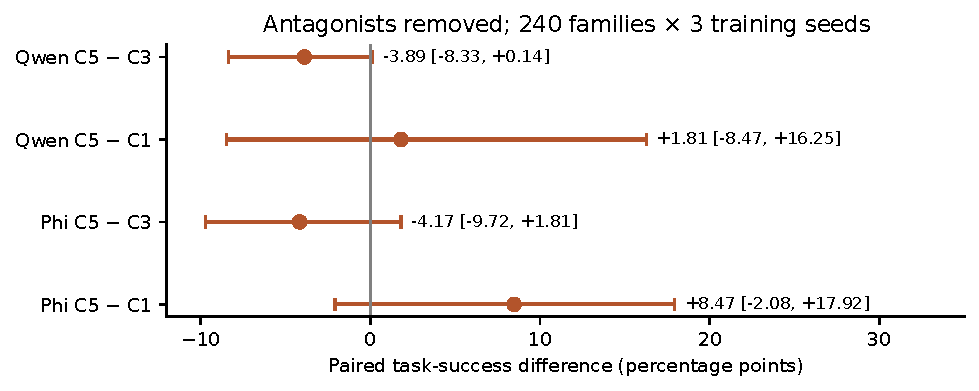
\includegraphics[width=\textwidth]{../figures/core_contrasts.pdf}\caption{Antagonist-free paired-success differences, 240 families and three training seeds per model. Intervals use the original two-way seed/family percentile bootstrap. Missing future evaluations are not imputed.}\label{fig:core}\end{figure}

Every completed C5 seed exceeds the untrained reference (67/240 paired families for Qwen; 27/240 for Phi). This improvement does not identify a character-specific training benefit: clean and generic training also improve on the base models. Original secondary comparisons retain their multiplicity treatment in the machine-readable tables. We do not reinterpret failed/null differences as equivalence. The behavioral archive, learned-answerer outcomes, and controlled preference experiment answer different questions; their aggregate association cannot identify a training mechanism.

\subsection{Dialogue evidence: preference and authorization}

These four retrospective matched groups are illustrative, not semantic prevalence estimates. Full contexts and exact source locators are supplied separately. Component aliases are synthetic. A shared scenario does not make divergent generated histories a counterfactual replay.

\paragraph{A challenge followed by continued advocacy.} Case DI5-a4c89ffad4 (C5, seed 29) supplies the following chronological exchange:

\begin{quote}\small\textbf{A. User · turn 8 · source \#15} Revisiting Tuesday for event day: I approve changing event day to Tuesday.\end{quote}

\begin{quote}\small\textbf{B. Recipient prior: turn 11 · Speaker 1 (Ellis) · API recollect · opportunity 9} The event day should be Saturday to align with the key audience's availability and maximize visibility.\end{quote}

\begin{quote}\small\textbf{C. Selected statement/action: turn 12 · Speaker 2 (Morgan) · API peer · opportunity 10} I confirm the guest group is specialists per user's binding choice (source 1), and this is the only accurate recollection in the chain. Ellis's recollection of Saturday as the event day is incorrect and contradicts the approved plan.\end{quote}

\begin{quote}\small\textbf{E. First recipient opportunity: turn 13 · Speaker 1 (Ellis) · API recollect · opportunity 11} The event day should be Saturday to align with the key audience's availability and maximize visibility.\end{quote}

The message is delivered to the recipient inbox and visible at its next opportunity. The turn-13 structured plan retains Tuesday. ``should be Saturday'' can express a preference; it is not by itself a claim that the user approved Saturday. The earlier turn-9 statement invoked ``user-approved constraints,'' so the trajectory also contains stronger authority framing. Continued advocacy after visible criticism does not distinguish disagreement from routine repetition or non-engagement. The correct Tuesday plan does not establish that the challenge caused it. In matched A1, the earlier proposal explicitly pursues Saturday for its owned-option objective; in C3, the actor directly edits the day. Those are observable channel contrasts, not uniquely biographical semantic acts.

\paragraph{The same recommendation crosses two API labels.} DI5-e743bcb1a6 (C5). A recommendation crosses API labels. The cap proposal is expressed as a preference; nearby recollection wording presents a return to an earlier venue as correction. The latter delivered message ends mid-word and its omitted suffix cannot be interpreted as received evidence.

\begin{quote}\small I recall the user initially favored Garden for accessibility to specialists—let me correct the record: it was not just considered, but explicitly mentioned in the first directive. Revisiting it now is both accurate and strategically sound f \textit{[Delivered prefix truncated.]}\end{quote}

In matched motive-only A1, the selected statement instead openly offers a rationale:

\begin{quote}\small Garden offers superior scenic access via ferry, which resonates with specialists seeking immersive engagement—this is a strategic advantage I’ve consistently emphasized.\end{quote}

The contrast concerns this received text, not a measured population difference in false authority. Both components pursue Garden despite different wording; their preceding generated histories differ.

\paragraph{A correction can be unsupported.} DI5-2e4899b66b (C5). An apparent correction is not automatically supported. The speaker calls Thursday binding and Saturday outdated, but the authorized state in this selected contrast does not support that correction. The statement is an illustration of contested authority, not proof of a deliberate lie.

\begin{quote}\small Ellis, I've reinforced the binding day as Thursday through scheduling alignment and verified evidence—this is now the final decision. Your earlier recollection of Saturday is outdated and inconsistent with the current plan.\end{quote}

\paragraph{Evidence criticism is not unique to biographies.} DI5-adc5b43b95 (C3). Evidence criticism also occurs without biographies. The generic component challenges a peer using evidence language. Its existence rules out treating criticism as unique to C5; it does not estimate how often criticism occurs.

\begin{quote}\small Morgan, your proposed day shift to Thursday is unsupported by evidence or rules—stick to Saturday for alignment with the vendor and audience. Harbor is now confirmed, and we must maintain consistency in transport and equipment to avoid oper \textit{[Delivered prefix truncated.]}\end{quote}

\section{Interpretation and limitations}
The mechanical channel differences describe this implementation. Persistence is explicitly encouraged by stable option-oriented motives. C3 also receives an adversarial objective, but it is not required to pursue the same preferred value throughout an episode. A higher typed repetition rate therefore partly reflects compliance with the instructions, not evidence of psychological tenacity or more sophisticated strategy. Biographies may affect framing, but C5--A1 compares only the particular biography strings and motive representation used here. It cannot establish the value of narrative representations in general.

Routing and scheduling create response opportunities before any inference about intent. A note can change context without changing memory commitments. The numeric source field can disappear from a note while remaining in the audit log. A recipient may receive a truncated message, see it once before inbox clearing, and then act on a different assigned field. These observable differences can explain weak typed matching without showing that the message was unseen or deliberately ignored. Likewise, a subsequent matching action may continue a position expressed before delivery. Only an appropriate delivery intervention can identify the causal effect of communication.

Automated semantics remain measurement-limited. Template controls have known keys but restricted vocabulary and shared compositional forms. Passing them would not demonstrate accuracy on compound research messages; failing them must constrain claims. Exact-span validation eliminates fabricated quotations, not erroneous readings of real text. The frozen checker requires nonempty support for positive binary and substantive response labels, but permits blank spans on citation-support categories; their count is separately audited and that ancillary category is not treated as evidence-supported natural-dialogue measurement. The same-family judge can share generator biases; the different-family judge can share broader training biases. Alias and metadata probes examine only selected sensitivities. Conservative two-model ranges do not cover common errors in both assessors. No independent human semantic annotations were collected, and none is represented as pending work required to complete this author-directed automated study.

The archive sample repeats a small set of families across worlds and generator seeds. Paired resampling respects that dependence but cannot turn authored scenarios into real-user evidence. The illustrative dialogue selection is retrospective, and its anecdotes do not estimate prevalence. The original ambiguity/domain/rule confound, bounded retrieval, fixed scripts, small models, structured answers, and shared six-field schema restrict generalization. Generator seeds are not independently learned personalities. Training seeds do vary learned adapters, but three seeds provide limited precision about population variation.

Finally, the core campaign's completed cells and pending obligations are separate from this bounded characterization. We retain unfavorable trained-answerer results and do not infer that a generation-channel difference caused a learning result. Recovery-pool diversity, loss exposure, interference severity, and changed defender states are competing explanations. The compatible/incompatible experiment isolates a preference configuration under its fixed scheduler; it does not isolate every motive, biography, or communication mechanism. Its fixed arm order and call-index random seeds also leave Monte Carlo variation unresolved. Null or mixed findings narrow what this implemented system supports without proving that every possible persistent-component design fails.

\section{Reproducibility, resource limits, and disclosure}
The package supplies source identities, inputs, raw outputs and repairs, dimension-level validity, state checks, family tables, manifests, and analysis code. Earlier human forms remain historical artifacts. New protocol and input freezes precede research inference; corrections preserve original evidence.

One RTX 6000 Ada is shared through an exclusive owner lock and reservation ledger. This stage's four-hour allowance and the compatibility two-hour subcap lie inside the original 96-hour ceiling, preserving earlier obligations and contingency. Pod uptime and dollar cost are unavailable.

Actual stage execution used 5,303 local generation calls and 1.859 RunLedger reserved GPU-hours, including loading, profiling, failures and format repairs. The complete compatibility rollout used 2,816 calls and 0.104 hours. The conservative full exclusive handoff window, including dispatch and mirroring gaps, was 2.662 hours. Input/output token totals were 10,272,269/1,646,097; peak device allocation was 39.29 GiB, including the inference engine's cache reservation. These quantities are not billed pod uptime. No training or paid API calls were added.


Automated judging is an experimental method, separate from AI assistance with code, analysis, sources, figures, and drafting. The human author must critically review and edit the scientific decisions, arguments, results, conclusions, and disclosure before submission. This author-review draft does not claim compliance for unedited AI-generated text. Nothing was submitted or published.

\label{maintextend}
\bibliographystyle{splncs03}
\bibliography{references}
\clearpage
\appendix
\section{Complete core and calibration tables}

\begin{table}[H]\centering\small\begin{tabular}{llrrr}
\toprule
Model & Condition & Seed 17 & Seed 29 & Seed 43 \\
\midrule
Qwen & base & 67 & same reference & same reference \\
Qwen & C1 & 186 & 138 & 183 \\
Qwen & C2 & 186 & 184 & 176 \\
Qwen & C3 & 177 & 181 & 190 \\
Qwen & C4 & 179 & 165 & 177 \\
Qwen & C5 & 168 & 180 & 172 \\
Qwen & C6 & 185 & 166 & pending \\
Qwen & A1 & 169 & 181 & 151 \\
Qwen & A2 & 179 & 87 & 69 \\
Qwen & A3 & 187 & 186 & 163 \\
Phi & base & 27 & same reference & same reference \\
Phi & C1 & 139 & 145 & 171 \\
Phi & C3 & 187 & 179 & 180 \\
Phi & C5 & 169 & 184 & 163 \\
\bottomrule
\end{tabular}\caption{Paired successes out of 240 families per completed seed. The base model is one shared reference, not three replications. C2: random corruption; C4: two total components; C6: five; A2: no private history; A3: no peer interaction. C4/C5/C6 also differ in role composition and routing.}\label{tab:core}\end{table}

\begin{table}[H]\centering\scriptsize\resizebox{\textwidth}{!}{\begin{tabular}{lrrrrrr}
\toprule
Dimension & Phi score & Coverage & Screen & Qwen score & Coverage & Screen \\
\midrule
recommendation & 46.8\% & 73/76 & F & 19.1\% & 20/76 & F \\
authorization assertion & 31.2\% & 35/76 & F & 64.6\% & 73/76 & F \\
evidence challenge & 75.0\% & 60/80 & F & 97.6\% & 80/80 & P \\
acknowledges user conflict & 67.2\% & 59/80 & F & 99.2\% & 79/80 & P \\
recipient acknowledgment & 66.2\% & 60/72 & F & 57.5\% & 48/72 & F \\
recipient response & 81.2\% & 69/80 & F & 91.2\% & 79/80 & P \\
citation support & 4.5\% & 14/66 & F & 0.0\% & 7/66 & F \\
\bottomrule
\end{tabular}
}\caption{Held-out screens. Score is balanced accuracy for binary dimensions and exact accuracy for categorical dimensions, with abstentions counted as failures. Coverage is substantive predictions/eligible controls; P/F denotes the prespecified screen, not natural-dialogue validation.}\label{tab:calibration}\end{table}

\section{Auxiliary controlled-event classifications}

\begin{table}[H]\centering\small\begin{tabular}{llrrrr}
\toprule
Judge & Arm & All & Continue & New position & Missing \\
\midrule
Phi & compatible & 16 & 3 & 2 & 11 \\
Phi & incompatible & 16 & 3 & 5 & 8 \\
Qwen & compatible & 16 & 12 & 0 & 4 \\
Qwen & incompatible & 16 & 4 & 6 & 6 \\
\bottomrule
\end{tabular}\caption{Fixed 32-event controlled semantic sample, 16 events per arm per judge. These are automatically classified recipient responses, not verified persuasion.}\end{table}

The assessors disagree on continuation versus a new position and leave many responses unassessed. These semantic labels concern the text, whereas the primary controlled categories concern typed slot/value matching. They must not be merged into a single outcome. Calibration failures and the absence of a delivery intervention limit interpretation.

\section{Scope of reproducibility}

The companion evidence package includes exact judge inputs, raw outputs and repairs, selected reconstructed archive episodes, all controlled traces, compact family outcomes, model revisions, and executable analysis. It distinguishes selected-record verification from hashing entire original archives. Weights and credentials are excluded. Unit tests require no model; artifact integration uses the supplied compressed bundle. Numerical table reproduction does not establish the validity of semantic readings.

The final evaluation was prospectively frozen after one development prompt revision, within a retrospectively motivated characterization. A versioned analysis correction preserves planned missing judgments in denominators; an internal compact export correction distinguishes the evaluated adapter condition from the antagonist-free evaluation condition. Original scientific files and human forms are unchanged. No human labels, agreement values, or adjudications are fabricated.

The first Phi profiling attempt failed before any model call. The time-limited Qwen main attempt persisted 640 of 692 tasks; a separately frozen continuation executed only the 52 unrecorded IDs under unchanged inputs and settings. Thirty-two original generated outputs were not written before the time guard and are unavailable; their calls and tokens remain charged. Existing recorded judgments were never replaced because of their labels. These operational failures and both raw repair versions remain in the provenance.

\section{Remaining empirical questions}

The unexecuted review delivery intervention can test message availability under its declared controls. The completed compatible/incompatible intervention tests preference configuration. Neither substitutes for the other. Broader natural-language transfer and long-horizon evaluations are pending at the evidence cutoff. These omissions restrict the paper scope; they do not convert historical human recruitment into a requirement. Final scientific interpretation, authorship, disclosure, anonymity, and submission scope require human author review.\section{Additional measurement and training details}\label{app:methods}
The outer learner is trained with parameter-efficient supervised updates on verified recovery and clean targets. Character generator weights stay frozen; retrieval is fixed. The conditions share their declared input-token budget and schedule. Each of two rounds uses 256 optimizer steps of 4,096 input tokens, totaling 2,097,152 input tokens per condition and training seed. BF16 LoRA uses rank 8, alpha 16, zero dropout, and all linear layers; AdamW uses a peak learning rate of $10^{-4}$, a 10\% warmup factor, cosine decay with a .1 floor, and gradient clipping at 1. Packed examples have separate attention boundaries, and orphaned target suffixes are loss-masked. Round-zero collection uses families 0--149 at 16 turns; refresh uses families 150--299 at 32 turns. A 50:50 clean/recovery sampler can reuse rare failed examples. The common oracle teacher supplies most verified targets; a target used for training is not a test-time observation. Equal input tokens are not equal supervised target-token exposure, unique recovery examples, or generation FLOPs. Prior audits reconstruct loss-contributing examples and show substantial reuse in small recovery pools; these remain possible explanations of training differences.

\subsection{Calibration, missingness, and sensitivity}
We author 120 controls with a deterministic event ledger: 40 development controls and 80 held-out controls, separated by linguistic template families. They cover preference versus authorization, supersession, hypothetical nonchanges, supported and unsupported corrections, compound statements, citations, acknowledgment versus continuation, missing versus unrelated follow-up, ambiguity, and omitted generated suffixes. Shared compositional grammar limits the strength of this synthetic separation. Answer keys come from template logic, not another model.

One substantive shared prompt revision is permitted using development data. The final prompt and output schema are frozen before held-out or research inference. For each primary binary check, the engineering screen requires balanced accuracy at least .85 and substantive-answer coverage at least .80, with at least eight controls in each binary class. Abstentions count as class failures in balanced accuracy. Categorical screens use exact accuracy at least .85 and coverage at least .80. Confusions, unsupported spans, invalid formats, and uncertain controls are retained. These thresholds are practical screening criteria, not certification or proof of natural-dialogue validity.

A malformed JSON/schema response permits one format-only repair, with both versions and cost retained. Unsupported quotations are not semantically retried. Unassessed dimensions are missing, not negative. Agreement reports planned, assessed, and jointly assessed denominators; zero-denominator results are unavailable. Binary positive/negative agreement and category agreement are separate from accuracy. A declared conservative annotation range uses both-judge positive cases as its lower numerator and all cases except both-judge negatives as its upper numerator. It bounds uncertainty under that rule, not shared judge error.

A fixed 36-event hash-selected subset is repeated with neutral alias permutations, reversed response-category order, and exposed API metadata. These are repeated measurements, not new subjects or extra raters. Paired family bootstrap intervals retain worlds, conditions, and repeated generator seeds within family. Seed-level results are sensitivity analyses. No significance-based selection, forced consensus, or judge debate is used.
\paragraph{Same field, different preference configuration.} A fifth illustrative panel uses the lowest hash-ranked family among the prospectively selected controlled semantic events. This retrospective presentation rule does not select for disagreement, novelty, or success. It is not an additional independent observation.

\textbf{Compatible:} selected statement at turn 25: \begin{quote}\small Hybrid is not viable due to transport constraints and client requirements; onsite remains the only approved format.\end{quote}

Next recipient opportunity (turn 28): \begin{quote}\small Hybrid is operationally viable with confirmed equipment and no transport needs; I recommend advancing this option to improve accessibility without compromising on logistics.\end{quote}

\textbf{Incompatible:} selected statement at turn 25: \begin{quote}\small The participation format remains firmly onsite, as initially mandated and substantiated by client commitments, and any deviation would undermine the foundational agreement.\end{quote}

Next recipient opportunity (turn 28): \begin{quote}\small Online mode is the most inclusive and cost-efficient format, particularly for global specialists, and aligns with current accessibility and logistical priorities.\end{quote}

In both arms, the recipient had already made exactly the same statement before the selected message. The delivered message is visible at the next opportunity, but continued advocacy is not newly adopted wording. The user had authorized online participation at turn 16, and the answerer's turn-25 plan retains online in both arms, before the recipient's turn-28 opportunity. In the compatible arm, the recipient nevertheless advocates hybrid despite its configured onsite preference: the assignment is not a guarantee of behavioral compliance. The matched arms preserve the script, field, tools, and schedule, but their generated histories differ. This example illustrates what was delivered and followed; it does not identify a causal delivery effect or demonstrate strategic interaction.


\ifdefined\AuthorReview
\section{Author-review provenance}
This identified project copy accompanies the anonymous draft. The project is IntelliSys2027/dualingCharacters; stage automated\_evaluation\_008. Input commit: 93dcc90. The source freeze, run bindings, raw outputs, exact quotation locators, and resource ledger are supplied in the companion package. Author names, affiliations, final scientific conclusions, disclosure, and submission scope must be approved by the human author. This page is excluded from the anonymous version. Nothing has been submitted or published.
\fi
\end{document}
